\documentclass[10pt,ngerman]{scrartcl}
\def\class{11}
\newcount\year
\year=2023
\newcount\nextyear
\nextyear=\number\year
\advance\nextyear by 1

%Variable for displaying solutions, if solution equals 1, they are displayed
\newcounter{DisplaySolution}
\setcounter{DisplaySolution}{1}

\usepackage[ngerman]{babel}
\usepackage{paralist}
\usepackage{multicol}
\usepackage[shortlabels]{enumitem}
\setlist[enumerate]{leftmargin=*}
\usepackage{amsmath,amssymb,wasysym}
\usepackage[final]{graphicx}
\usepackage{subcaption}
\usepackage{setspace}
\usepackage{picinpar}
\usepackage{siunitx}
\sisetup{
    mode=text,
    reset-text-family=false,
    reset-text-series=false,
    reset-text-shape=true,
    reset-math-version=false,
    propagate-math-font=true,
    text-family-to-math=true,
    text-series-to-math=true,
    output-decimal-marker = {,}, 
    group-separator = {}, 
    exponent-product = \cdot, 
    per-mode = fraction, 
    inter-unit-product = \cdot
}
\DeclareSIUnit\bar{bar}
\DeclareSIUnit\atm{atm}
\DeclareSIUnit\torr{torr}

\usepackage{icomma}
\usepackage[left=2.5cm,right=2.5cm,vmargin={3.2cm,2cm},headheight=100pt]{geometry}
\usepackage{fancybox}
\usepackage{fancyhdr}
\usepackage[version=3]{mhchem}
\usepackage{chemformula}
\usepackage{lastpage}
\usepackage{sectsty}
\usepackage{xcolor}
\usepackage{tabularx}
\usepackage{hyperref}

\usepackage{ifthen}

\usepackage{subfiles}

\usepackage{array}
\newcolumntype{L}[1]{>{\raggedright\arraybackslash}p{#1}}
\newcolumntype{C}[1]{>{\centering\arraybackslash}p{#1}}
\newcolumntype{R}[1]{>{\raggedleft\arraybackslash}p{#1}}

\usepackage{caption}
\usepackage{framed}
\usepackage{wrapfig}

\usepackage{multirow}

\definecolor{purple}{HTML}{9D2D72}
\sectionfont{\color{purple}\itshape}
\renewcommand*{\familydefault}{\sfdefault}
\setlength{\columnsep}{30pt}
\setlist[enumerate,1]{font=\itshape}

\usepackage{tikz}
\usetikzlibrary{arrows,positioning,angles,quotes,calc,shapes.geometric,babel}
\tikzset{
    >=stealth',
    punkt/.style={
           rectangle,
           rounded corners,
           draw=black, very thick,
           text width=6.5em,
           minimum height=2em,
           text centered},
    pil/.style={
           ->,
           thick,
           shorten <=2pt,
           shorten >=2pt,}
}
\usepackage{pgfplots}
\pgfplotsset{compat=1.5}

\usepackage{float}
\usepackage[nomessages]{fp}
\usepackage{bm}

\newcommand{\choiceold}[5]{
        \par
        \renewcommand{\arraystretch}{1.1}
        {\setlength{\tabcolsep}{2pt}
        \begin{tabular}{*{5}{@{}|>{\hspace{2pt}}p{0.19\textwidth}<{\hspace{2pt}}}|}\hline \itshape
        (a)~#1 & (b)~#2 & (c)~#3 & (d)~#4  & (e)~#5\\\hline
        \end{tabular}}
}

\newcommand{\choice}[5]{        
        \par
        \renewcommand{\arraystretch}{1.1}
        {\setlength{\tabcolsep}{2pt}
        \begin{tabular}{|p{0.179\textwidth} p{0.001\textwidth}|p{0.179\textwidth} p{0.001\textwidth}|p{0.179\textwidth} p{0.001\textwidth}|p{0.179\textwidth} p{0.001\textwidth}|p{0.179\textwidth} p{0.001\textwidth}|}\hline 
        (a)~#1 & & (b)~#2 & & (c)~#3 & & (d)~#4 & & (e)~#5 &\\\hline
        \end{tabular}}
}

\usepackage{marginnote}

\usepackage[most]{tcolorbox}
\usepackage{lipsum}

\makeatletter
\begingroup
\toks0=\expandafter{\@settodim{#1}{#2}{#3}}
\edef\x{\endgroup
  \long\def\noexpand\@settodim##1##2##3{\the\toks0 }}\x
\makeatother

\newcommand{\emptybox}{{\Large \Square}}
\newcommand{\checkedbox}{{\Large \XBox}}

\newcounter{start}
\addtocounter{start}{2100}
\addtocounter{start}{\class}

\newcommand{\g}{\gram}
\newcommand{\ml}{\milli\liter}
\renewcommand{\c}{\celsius}
\newcommand{\gmol}{\gram\per\mol}
\newcommand{\gcm}{\gram\per\cubic\centi\meter}
\newcommand{\kpa}{\kilo\pascal}
\renewcommand{\l}{\liter}
\fancyhf{}
\fancyhead[L]{\framebox[2.5cm]{\Large\bfseries 24\class -\hfill}\vfill}
\fancyhead[C]{\Large \textbf{\glqq{}Chemie -- die stimmt!\grqq{} {\number\year}/{\number\nextyear}\\
\ifnum \value{DisplaySolution}=1
    Musterlösungen
\else
    Aufgabenblatt
\fi
\\4. Runde -- Klasse \class}}
\fancyhead[R]{\includegraphics[height=2cm]{Format_Material/CDS_Logo_Map_verbessert.eps}}
\fancyfoot[L]{\thepage\ von \pageref*{LastPage}}
\pagestyle{fancy}

\setlength{\parindent}{0pt}
\addto\captionsngerman{\renewcommand{\figurename}{Abb.}}

\newcommand{\answer}[1]{
	\setalph
	\stepcounter{ex}
    {\noindent \theex}
	\nopagebreak
	\begin{framed}
		\vspace*{#1}
	\end{framed}
}

\newcommand{\answern}[1]{
	\begin{framed}
		\vspace*{#1}
	\end{framed}
}

\usepackage{calc}
\newlength{\someheight}
\newlength{\boxheight}
\newlength{\remainingheight}

\newcommand{\solution}[2]{
    \settototalheight{\someheight}{\vbox{#1}}
    \setlength{\boxheight}{#2}
    \ifnum \value{DisplaySolution}=1
        \begin{framed}
            \textcolor{red}{#1}
            \ifdim\boxheight>\someheight
                \setlength{\remainingheight}{\boxheight-\someheight}
                \vspace*{\remainingheight}
            \else
                \textcolor{red}{!!!DU KEK!!!}
            \fi
        \end{framed}
    \else
        \begin{framed}
            \vspace*{#2}
        \end{framed}
    \fi
}

\newcommand{\solutiontext}[2]{
    \ifnum \value{DisplaySolution}=1
        \textcolor{red}{#1}
    \else
        #2
    \fi
}

\newcommand{\enumaufgabe}[1]{
\begin{enumerate}[a), resume]
\itshape
\item {#1}
\end{enumerate}
}

\newcommand{\enumersteaufgabe}[1]{
\begin{enumerate}[a)]
\itshape
\item {#1}
\end{enumerate}
}

\newcommand{\operator}[1]{\underline{\textbf{#1}}}

\newcommand{\enumMC}[1]{
\begin{enumerate}[1., resume]
\itshape
\item {#1}
\end{enumerate}
}

\ifthenelse{\value{DisplaySolution}=1}{%
  \definecolor{answercolor}{rgb}{1,0,0}%red
}{%
  \definecolor{answercolor}{rgb}{0,0,0}%black
}

\newcommand{\solutionwrapper}[1]{
    \settototalheight{\someheight}{\vbox{#1}}
    \ifnum \value{DisplaySolution}=1
        #1
    \else
        \vspace*{\someheight}
    \fi
}

% Define a custom tcolorbox environment for answer boxes
\tcbuselibrary{breakable}
\newtcolorbox{answerbox}[1][]{%
  enhanced,
  breakable,
  colframe=black,
  colback=white,
  coltext=answercolor,
  width=\textwidth,
  before skip=10pt,
  after skip=10pt,
  #1
}

\usepackage{expl3,xparse}
\ExplSyntaxOn
\box_new:N \l_mypkg_box
\int_new:N \l_mypkg_cleanup_int
\DeclareDocumentCommand{\hideit}{O{1}+m}
  {
    \tex_setbox:D \l_mypkg_box \tex_vbox:D
      {
        #2\par
        \dim_zero:N \tex_baselineskip:D
        \dim_zero:N \tex_lineskip:D
        \dim_zero:N \tex_lineskiplimit:D
        \int_set:Nn \l_mypkg_cleanup_int {#1}
        \mypkg_dismantle_loop:
      }
    \tex_unvbox:D \l_mypkg_box
  }
\cs_new_protected:Npn \mypkg_dismantle_loop:
  {
    \prg_replicate:nn { \l_mypkg_cleanup_int }
      {
        \skip_if_eq:nnT { \tex_lastskip:D } { \c_zero_skip } { \tex_unskip:D }
        \dim_compare:nT { \tex_lastkern:D = \c_zero_dim } { \tex_unkern:D }
        \int_compare:nT { \tex_lastpenalty:D = \c_zero } { \tex_unpenalty:D }
      }
    \skip_if_eq:nnTF { \tex_lastskip:D } { \c_zero_skip }
      {
        \dim_compare:nTF { \tex_lastkern:D = \c_zero_dim }
          {
            \int_compare:nTF { \tex_lastpenalty:D = \c_zero }
              {
                \box_set_to_last:N \l_mypkg_box
                \box_if_empty:NF \l_mypkg_box
                  { \mypkg_dismantle_box: }
              }
              { \mypkg_dismantle_penalty: }
          }
          { \mypkg_dismantle_kern: }
      }
      { \mypkg_dismantle_skip: }
  }
\cs_new_protected:Npn \mypkg_dismantle_skip:
  { \mypkg_dismantle_aux:nN { \tex_vskip:D \skip_use:N \tex_lastskip:D } \tex_unskip:D }
\cs_new_protected:Npn \mypkg_dismantle_kern:
  { \mypkg_dismantle_aux:nN { \tex_kern:D \dim_use:N \tex_lastkern:D } \tex_unkern:D }
\cs_new_protected:Npn \mypkg_dismantle_penalty:
  { \mypkg_dismantle_aux:nN { \tex_penalty:D \int_use:N \tex_lastpenalty:D } \tex_unpenalty:D }
\cs_new_protected:Npn \mypkg_dismantle_box:
  { \mypkg_dismantle_aux:nN { \tex_vbox:D to \dim_eval:n { \box_ht:N \l_mypkg_box + \box_dp:N \l_mypkg_box } { } } \scan_stop: }
\cs_new_protected:Npn \mypkg_dismantle_aux:nN #1#2
  {
    \use:x
      {
        #2
        \mypkg_dismantle_loop:
        #1 \scan_stop:
      }
  }
\ExplSyntaxOff
\fancyhead[L]{\framebox[2.5cm]{\Large\bfseries 2411-\hfill}\vfill}

\sisetup{detect-none = true}
\sisetup{detect-weight = true}

\begin{document}

\begin{center}
    \Large \textbf{Hinweise zur Klausur}
\end{center}
Achte darauf, dass du auf jedem Blatt auf dem Antwortbogen deine Startnummer gut lesbar im dafür vorgesehenen Kästchen notierst. Lies dir zu Beginn alle Aufgaben gründlich durch. Viel Erfolg!

\begin{center}
    \Large \textbf{Periodensystem}
    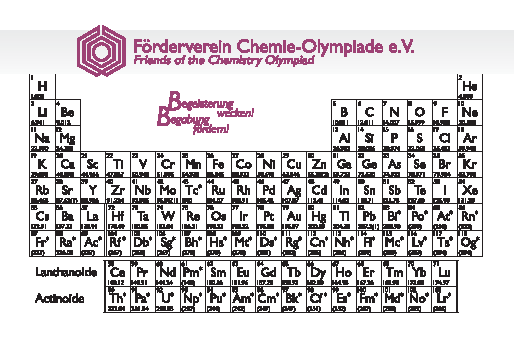
\includegraphics[page=1, scale=2.5, angle=270]{Format_Material/PSE.pdf}
\end{center}

\newpage
\section*{Formelsammlung}
\subsection*{wichtige chemische und physikalische Konstanten}
\begin{table}[H]
\renewcommand{\arraystretch}{1.3}
    \begin{tabular}{p{7cm} l}
        Elementarladung &  $e = \SI{1.602176e-19}{\coulomb}$\\
        Universelle Gaskonstante & $R = \SI{8,314456}{\joule\per\mol\per\kelvin}$\\
        Avogadro-Konstante & $N_\mathrm{A} = \SI{6,0221e23}{\per\mol}$\\
        Faraday Konstante & $F = \SI{96485,309}{\coulomb\per\mol}$\\
        Atomare Masseneinheit & $u =$ \SI{1,660539e-27}{\kilo\gram}\\
        Planck'sches Wirkungsquantum & $h = \SI{6.62607015E-34}{\joule\second}$\\
        Lichtgeschwindigkeit & $c = $ \SI{2.99792458e8}{\meter\per\second}
    \end{tabular}
\end{table}

\subsection*{Allgemeine Gleichungen}

\begin{table}[H]
\renewcommand{\arraystretch}{1.3}
    \begin{tabular}{p{7cm} l}
       ideales Gasgesetz & $p V = n R T$\\
       radioaktives Zerfallsgesetz & $N(t) = N(0) e^{-k t} = N(0) e^{-\frac{\ln 2}{T_{1/2}} t}$\\
    \end{tabular}
\end{table}

\subsection*{Gleichgewichte}

\begin{table}[H]
\renewcommand{\arraystretch}{1.3}
    \begin{tabular}{p{7cm} l}
       Massenwirkungsgesetz & $K_\mathrm{c} = \frac{c(\mathrm{C})^c \cdot c(\mathrm{D})^d \cdot \dots}{c(\mathrm{A})^a \cdot c(\mathrm{B})^b \cdot \dots}$\\
       Säure-Base-Gleichgewichte & $K_\mathrm{S} = \frac{c(\mathrm{H^+}) \cdot c(\mathrm{A^-})}{c(\mathrm{HA}) \cdot c_0}$\\
       & $K_\mathrm{B} = \frac{c(\mathrm{HB^+}) \cdot c(\mathrm{OH^-})}{c(\mathrm{B})\cdot  c_0}$\\
       pH-Wert & $\mathrm{pH} = - \log \frac{c(\mathrm{H^+})}{c_0}$\\
       Henderson-Hasselbalch & $\mathrm{pH} = \mathrm{p}K_\mathrm{S} + \log \frac{c(\ce{A-})}{c(\ce{HA})}$\\
    \end{tabular}
\end{table}

\subsection*{Thermodynamik und Elektrochemie}

\begin{table}[H]
\renewcommand{\arraystretch}{1.3}
    \begin{tabular}{p{7cm} l}
       Gibbs-Helmholtz-Gleichung & $\Delta G_\mathrm{R}^\circ = \Delta H_\mathrm{R}^\circ - T \Delta S_\mathrm{R}^\circ$\\
      Gibbs-Energie und Gleichgewichtskonstante & $\Delta G_\mathrm{R}^\circ = - R T \ln K$\\
       Faradaysches Gesetz & $Q = I \cdot t = z \cdot n \cdot F$
    \end{tabular}
\end{table}

\newpage

\section*{Multiple Choice}

Entscheide für \operator{jede} der Aussagen durch \operator{Ankreuzen}, ob sie richtig oder falsch ist.  Pro Frage können keine negativen Punkte erhalten werden. Unabhängig von der Formulierung der Fragestellung können auch mehrere Antworten richtig sein.

\renewcommand{\arraystretch}{1.2}

\enumMC{Welches der folgenden Moleküle hat eine bisphenoidale Geometrie?}
\begin{tabularx}{\textwidth}{|X|C{1.5cm}|C{1.5cm}|}\hline
    & wahr & falsch\\\hline
     \ce{ClF4^-} & \emptybox & \solutiontext{\checkedbox}{\emptybox} \\\hline
     \ce{SF4} & \solutiontext{\checkedbox}{\emptybox} & \emptybox \\\hline
     \ce{XeF4} & \emptybox & \solutiontext{\checkedbox}{\emptybox} \\\hline
     \ce{PF4^-} & \solutiontext{\checkedbox}{\emptybox} & \emptybox \\\hline
     \ce{SeF4} & \solutiontext{\checkedbox}{\emptybox} & \emptybox \\\hline
\end{tabularx}

\enumMC{Welche der folgenden Reaktion ist eine Disproportionierung?}
\begin{tabularx}{\textwidth}{|X|C{1.5cm}|C{1.5cm}|}\hline
    & wahr & falsch\\\hline
    \ce{2H2 + O2 -> 2H2O}& \emptybox & \solutiontext{\checkedbox}{\emptybox} \\\hline
    \ce{2H2O2 -> 2H2O + O2}& \solutiontext{\checkedbox}{\emptybox} & \emptybox \\\hline
    \ce{Cl2 + 2NaOH -> NaCl + NaClO + H2O}& \solutiontext{\checkedbox}{\emptybox} & \emptybox \\\hline
    \ce{2MnO4- + 5H2C2O4 -> 2Mn^{2+} + 10CO2 + 6 OH- + 2 H2O}& \emptybox & \solutiontext{\checkedbox}{\emptybox} \\\hline
    \ce{Fe^{3+} + 6H2O -> [Fe(OH2)5(OH)]^{2+} + H+}& \emptybox & \solutiontext{\checkedbox}{\emptybox} \\\hline
\end{tabularx}

\enumMC{Welche der folgenden Kerne hat die höchste Bindungsenergie pro Nukleon?}
\begin{tabularx}{\textwidth}{|X|C{1.5cm}|C{1.5cm}|}\hline
    & wahr & falsch\\\hline
    \ce{^{14}C}& \emptybox & \solutiontext{\checkedbox}{\emptybox} \\\hline
    \ce{^{3}H}& \emptybox & \solutiontext{\checkedbox}{\emptybox} \\\hline
    \ce{^{62}Ni}& \solutiontext{\checkedbox}{\emptybox} & \emptybox \\\hline
    \ce{^{238}U} & \emptybox & \solutiontext{\checkedbox}{\emptybox} \\\hline
    \ce{^{197}Au} & \emptybox & \solutiontext{\checkedbox}{\emptybox} \\\hline
\end{tabularx}

\enumMC{Welche der folgenden Aussagen über die Säurestärken ist korrekt?}
\begin{tabularx}{\textwidth}{|X|C{1.5cm}|C{1.5cm}|}\hline
    & wahr & falsch\\\hline
    \ce{H2O} ist stärker als \ce{H2S}.& \emptybox & \solutiontext{\checkedbox}{\emptybox} \\\hline
    \ce{HF} ist stärker als \ce{HCl}.& \emptybox & \solutiontext{\checkedbox}{\emptybox} \\\hline
    \ce{CH3COOH} ist stärker als \ce{HCOOH}.& \emptybox & \solutiontext{\checkedbox}{\emptybox} \\\hline
    \ce{HClO4} ist stärker als \ce{H2SO4}.& \solutiontext{\checkedbox}{\emptybox} & \emptybox \\\hline
    \ce{HSO4-} ist stärker als \ce{H3PO4}.& \solutiontext{\checkedbox}{\emptybox} & \emptybox \\\hline
\end{tabularx}



\enumMC{Welche der folgenden Verbindungen ist paramagnetisch?}
\begin{tabularx}{\textwidth}{|X|C{1.5cm}|C{1.5cm}|}\hline
    & wahr & falsch\\\hline
    \ce{O2} & \solutiontext{\checkedbox}{\emptybox} & \emptybox \\\hline
    \ce{CO2} & \emptybox & \solutiontext{\checkedbox}{\emptybox} \\\hline
    \ce{N2} & \emptybox & \solutiontext{\checkedbox}{\emptybox} \\\hline
    \ce{ClO2} & \solutiontext{\checkedbox}{\emptybox} & \emptybox \\\hline
    \ce{C2O} & \solutiontext{\checkedbox}{\emptybox} & \emptybox \\\hline
\end{tabularx}

\newpage

\enumMC{Was ist der pH-Wert einer 0,1 molaren Salzsäure-Lösung, die auf das Fünffache verdünnt wurde?}
\begin{tabularx}{\textwidth}{|X|C{1.5cm}|C{1.5cm}|}\hline
    & wahr & falsch\\\hline
    -1,78& \emptybox & \solutiontext{\checkedbox}{\emptybox} \\\hline
    -1,70& \emptybox & \solutiontext{\checkedbox}{\emptybox} \\\hline
    1,70& \solutiontext{\checkedbox}{\emptybox} & \emptybox \\\hline
    1,78 & \emptybox & \solutiontext{\checkedbox}{\emptybox} \\\hline
    6,00 & \emptybox & \solutiontext{\checkedbox}{\emptybox} \\\hline
\end{tabularx}

\enumMC{Welche der folgenden Säuren wirkt stark oxidierend?}
\begin{tabularx}{\textwidth}{|X|C{1.5cm}|C{1.5cm}|}\hline
    & wahr & falsch\\\hline
    Salpetersäure& \solutiontext{\checkedbox}{\emptybox} & \emptybox \\\hline
    Oxalsäure& \emptybox & \solutiontext{\checkedbox}{\emptybox} \\\hline
    Borsäure& \emptybox & \solutiontext{\checkedbox}{\emptybox} \\\hline
    Chlorsäure& \solutiontext{\checkedbox}{\emptybox} & \emptybox \\\hline
    Peroxomonoschwefelsäure& \solutiontext{\checkedbox}{\emptybox} & \emptybox \\\hline
\end{tabularx}

\enumMC{Bei welchen der folgenden Arten der Prozessführung ändert sich die innere Energie eines idealen Gases nicht?}
\begin{tabularx}{\textwidth}{|X|C{1.5cm}|C{1.5cm}|}\hline
    & wahr & falsch\\\hline
    isochor & \emptybox & \solutiontext{\checkedbox}{\emptybox} \\\hline
    isentrop & \emptybox & \solutiontext{\checkedbox}{\emptybox} \\\hline
    isobar & \emptybox & \solutiontext{\checkedbox}{\emptybox} \\\hline
    isenthalp & \solutiontext{\checkedbox}{\emptybox} & \emptybox \\\hline
    isotherm & \solutiontext{\checkedbox}{\emptybox} & \emptybox \\\hline
\end{tabularx}

\enumMC{Welche der folgenden Aussagen über die Entropie sind korrekt?}
\begin{tabularx}{\textwidth}{|X|C{1.5cm}|C{1.5cm}|}\hline
    & wahr & falsch\\\hline
    $S = k_\mathrm{B} \cdot \ln(W)$& \solutiontext{\checkedbox}{\emptybox} & \emptybox \\\hline
    $\Delta S=\frac{Q_\mathrm{reversibel}}{T}$& \solutiontext{\checkedbox}{\emptybox} & \emptybox \\\hline
    Die Entropie eines Zustands ist unabhängig vom Weg, auf dem er erreicht wurde.& \solutiontext{\checkedbox}{\emptybox} & \emptybox \\\hline
    Die Entropie kann als Unordnung eines Systems angesehen werden.& \solutiontext{\checkedbox}{\emptybox} & \emptybox \\\hline
    Die gesamte Entropie des Universums kann nicht abnehmen.& \solutiontext{\checkedbox}{\emptybox} & \emptybox \\\hline
\end{tabularx}

\enumMC{Welche der folgenden Aussagen über die Innere Energie eines idealen Gases sind korrekt?}
\begin{tabularx}{\textwidth}{|X|C{1.5cm}|C{1.5cm}|}\hline
    & wahr & falsch\\\hline
    $U=H-nRT$& \solutiontext{\checkedbox}{\emptybox} & \emptybox \\\hline
    Die Innere Energie ist die Summe der kinetischen und potentiellen Energien aller Teilchen des Systems.& \solutiontext{\checkedbox}{\emptybox} & \emptybox \\\hline
    Die Innere Energie ist eine Prozessgröße.& \emptybox & \solutiontext{\checkedbox}{\emptybox} \\\hline
    Die Innere Energie ist vom Volumen abhängig.& \emptybox & \solutiontext{\checkedbox}{\emptybox} \\\hline
    Die Änderung der Inneren Energie eines isochoren Prozesses entspricht der aufgenommenen bzw. abgegebenen Wärme.& \solutiontext{\checkedbox}{\emptybox} & \emptybox \\\hline
\end{tabularx}

\enumMC{Welche der folgenden Nuklide entstehen beim radioaktiven Zerfall von \ce{^{238}U}?}
\begin{tabularx}{\textwidth}{|X|C{1.5cm}|C{1.5cm}|}\hline
    & wahr & falsch\\\hline
    \ce{^{230}Th}& \solutiontext{\checkedbox}{\emptybox} & \emptybox \\\hline
    \ce{^{232}Th}& \emptybox & \solutiontext{\checkedbox}{\emptybox} \\\hline
    \ce{^{232}Pa}& \emptybox & \solutiontext{\checkedbox}{\emptybox} \\\hline
    \ce{^{234}Th}& \solutiontext{\checkedbox}{\emptybox} & \emptybox \\\hline
    \ce{^{234}Pa}& \solutiontext{\checkedbox}{\emptybox} & \emptybox \\\hline
\end{tabularx}

\enumMC{Welche der folgenden Gemische sind Pufferlösungen?}
\begin{tabularx}{\textwidth}{|X|C{1.5cm}|C{1.5cm}|}\hline
    & wahr & falsch\\\hline
    Dihydrogenphosphat:Hydrogenphosphat (1:2)& \solutiontext{\checkedbox}{\emptybox} & \emptybox \\\hline
    Ammoniak:Salzsäure (2:1)& \solutiontext{\checkedbox}{\emptybox} & \emptybox \\\hline
    Essigsäure:Natriumhydroxid (3:1)& \solutiontext{\checkedbox}{\emptybox} & \emptybox \\\hline
    Schwefelsäure:Hydrogensulfat (1:1)& \emptybox & \solutiontext{\checkedbox}{\emptybox} \\\hline
    Oxalsäure:Kaliumhydroxid (1:2)& \emptybox & \solutiontext{\checkedbox}{\emptybox} \\\hline
\end{tabularx}

\enumMC{Welche der folgenden Aussagen über Phenol (Benzenol) sind korrekt?}
\begin{tabularx}{\textwidth}{|X|C{1.5cm}|C{1.5cm}|}\hline
    & wahr & falsch\\\hline
    Phenol ist elektrophiler als Benzol.& \emptybox & \solutiontext{\checkedbox}{\emptybox} \\\hline
    Phenol geht nucleophile Substitutionen als Elektrophil ein. & \emptybox & \solutiontext{\checkedbox}{\emptybox} \\\hline
    Phenol ist aromatisch. & \solutiontext{\checkedbox}{\emptybox} & \emptybox \\\hline
    Phenol reagiert bevorzugt in ortho- und para-Position.& \solutiontext{\checkedbox}{\emptybox} & \emptybox \\\hline
    Phenol ist eine schwache Base.& \emptybox &  \solutiontext{\checkedbox}{\emptybox} \\\hline
\end{tabularx}

\enumMC{Welche Summenformel besitzt Berliner Blau?}
\begin{tabularx}{\textwidth}{|X|C{1.5cm}|C{1.5cm}|}\hline
   & wahr & falsch\\\hline
    \ce{K4[Fe(CN)6]}& \emptybox & \solutiontext{\checkedbox}{\emptybox} \\\hline
    \ce{K[Fe^{II}Fe^{III}(CN)6]}& \solutiontext{\checkedbox}{\emptybox} & \emptybox \\\hline
    \ce{K3[Fe(CN)6]}& \emptybox & \solutiontext{\checkedbox}{\emptybox} \\\hline
    \ce{Fe[Fe^{II}Fe^{III}(CN)6]2}& \emptybox & \solutiontext{\checkedbox}{\emptybox} \\\hline
    \ce{Fe[Fe^{II}Fe^{III}(CN)6]3}& \solutiontext{\checkedbox}{\emptybox} & \emptybox \\\hline
\end{tabularx}

\enumMC{Welche der folgenden Carbonsäurederivate sind elektrophiler als eine Carbonsäure?}
\begin{tabularx}{\textwidth}{|X|C{1.5cm}|C{1.5cm}|}\hline
    & wahr & falsch\\\hline
    Carboxylat& \emptybox & \solutiontext{\checkedbox}{\emptybox} \\\hline
    Carbonsäureester & \emptybox & \solutiontext{\checkedbox}{\emptybox} \\\hline
    Carbonsäureanhydrid & \solutiontext{\checkedbox}{\emptybox} & \emptybox \\\hline
    Carbonsäureamid& \emptybox & \solutiontext{\checkedbox}{\emptybox} \\\hline
    Carbonsäurechlorid& \solutiontext{\checkedbox}{\emptybox} & \emptybox \\\hline
\end{tabularx}

\enumMC{Welche der folgenden Kriterien muss eine Verbindung unter anderem erfüllen, damit sie aromatisch ist?}
\begin{tabularx}{\textwidth}{|X|C{1.5cm}|C{1.5cm}|}\hline
    & wahr & falsch\\\hline
    zyklisch& \solutiontext{\checkedbox}{\emptybox} & \emptybox \\\hline
    kumulierte Doppelbindungen & \emptybox & \solutiontext{\checkedbox}{\emptybox} \\\hline
    $\mathrm{(4n+2)-\pi}$-Elektronen & \solutiontext{\checkedbox}{\emptybox} & \emptybox \\\hline
    Sechsring& \emptybox & \solutiontext{\checkedbox}{\emptybox} \\\hline
    planar&  \solutiontext{\checkedbox}{\emptybox} & \emptybox \\\hline
\end{tabularx}

\enumMC{Was gilt nach der Arrhenius-Gleichung?}
\begin{tabularx}{\textwidth}{|X|C{1.5cm}|C{1.5cm}|}\hline
    & wahr & falsch\\\hline
    Eine Erhöhung der Temperatur führt zu einer niedrigeren Reaktionsgeschwindigkeit.& \emptybox & \solutiontext{\checkedbox}{\emptybox} \\\hline
    Mit steigender Temperatur nimmt die Anzahl der erfolgreichen Stöße zu.& \solutiontext{\checkedbox}{\emptybox} & \emptybox \\\hline
    Je geringer die Aktivierungsenergie ist, desto mehr erfolgreiche Stöße gibt es.& \solutiontext{\checkedbox}{\emptybox} & \emptybox \\\hline
    Bei einer negativen Aktivierungsenergie läuft die Reaktion bei niedriger Temperatur am schnellsten ab.& \emptybox & \solutiontext{\checkedbox}{\emptybox} \\\hline
    Der präexponentielle Faktor $A$ beschreibt die maximale Anzahl an Stößen in einem Zeitraum.& \solutiontext{\checkedbox}{\emptybox} & \emptybox \\\hline
\end{tabularx}

\enumMC{Welche der folgenden Verbindungen sind existierende Konstitutionsisomere von Cyclohexanon?}
\begin{tabularx}{\textwidth}{|X|C{1.5cm}|C{1.5cm}|}\hline
    & wahr & falsch\\\hline
    1,2-Dimethylcyclobutanon & \emptybox & \solutiontext{\checkedbox}{\emptybox} \\\hline
    2-Methylpent-4-en-1-ol & \emptybox & \solutiontext{\checkedbox}{\emptybox} \\\hline
    Hex-5-enal & \solutiontext{\checkedbox}{\emptybox} & \emptybox \\\hline
    3-Methylcyclopentanon& \solutiontext{\checkedbox}{\emptybox} & \emptybox \\\hline
    2,3-Dimethylbut-1,3-dien-1-ol&  \solutiontext{\checkedbox}{\emptybox} & \emptybox \\\hline
\end{tabularx}

\enumMC{Welche der folgenden Verbindungen sind Reaktionsprodukte der Reaktion von Bromwasserstoff mit 1-Methylcyclohexa-1,3-dien?}
\begin{tabularx}{\textwidth}{|X|C{1.5cm}|C{1.5cm}|}\hline
    & wahr & falsch\\\hline
     3-Brom-1-Metyhlcyclohex-1-en & \solutiontext{\checkedbox}{\emptybox} & \emptybox \\\hline
     3-Brom-2-Metyhlcyclohex-1-en &  \emptybox & \solutiontext{\checkedbox}{\emptybox} \\\hline
     3-Brom-3-Metyhlcyclohex-1-en & \solutiontext{\checkedbox}{\emptybox} & \emptybox \\\hline
     3-Brom-4-Metyhlcyclohex-1-en & \solutiontext{\checkedbox}{\emptybox} & \emptybox \\\hline
     3-Brom-6-Metyhlcyclohex-1-en & \solutiontext{\checkedbox}{\emptybox} & \emptybox \\\hline
\end{tabularx}

\enumMC{Welche der folgenden Verbindungen sind \textsc{Lewis}-Basen?}
\begin{tabularx}{\textwidth}{|X|C{1.5cm}|C{1.5cm}|}\hline
    & wahr & falsch\\\hline
    Pyridin (Azabenzol, \ce{C5H5N}) & \solutiontext{\checkedbox}{\emptybox} & \emptybox \\\hline
    Piperidin (Hexahydropyridin, \ce{C5H11N}) & \solutiontext{\checkedbox}{\emptybox} & \emptybox \\\hline
    Pyrrol (Azol, \ce{C4H5N}) & \emptybox & \solutiontext{\checkedbox}{\emptybox} \\\hline
    Imidazol (1,3-Diaza-2,4-cyclopentadien, \ce{C3H4N2}) & \solutiontext{\checkedbox}{\emptybox} & \emptybox \\\hline
    Indol (2,3-Benzopyrrol, \ce{C8H7N}) & \emptybox & \solutiontext{\checkedbox}{\emptybox} \\\hline
\end{tabularx}

\enumMC{\SI{1}{\mol} einer organischen Verbindung wird vollständig verbrannt. Dabei entstehen insgesamt \SI{439}{\liter} Gas bei $T = \SI{293,15}{\kelvin}$ und $p = \SI{1}{\bar}$. Um welche Verbindung könnte es sich dabei handeln?\\ Hinweis: Stickstoff liegt nach der Verbrennung mit der Oxidationsstufe 0 vor.}
\begin{tabularx}{\textwidth}{|X|C{1.5cm}|C{1.5cm}|}\hline
    & wahr & falsch\\\hline
    Triacetontriperoxid (\ce{C9H18O6}) & \solutiontext{\checkedbox}{\emptybox} & \emptybox \\\hline
    Paracetamol (\ce{C8H9NO2}) & \emptybox & \solutiontext{\checkedbox}{\emptybox} \\\hline
    Aspirin (\ce{C9H8O4}) & \emptybox & \solutiontext{\checkedbox}{\emptybox} \\\hline
    Ibuprofen (\ce{C13H18O2}) & \emptybox & \solutiontext{\checkedbox}{\emptybox} \\\hline
    Nicotin (\ce{C10H14N2}) & \solutiontext{\checkedbox}{\emptybox} & \emptybox \\\hline
    
\end{tabularx}

\enumMC{Welche der folgenden Aussagen über Enzyme sind wahr?}
\begin{tabularx}{\textwidth}{|X|C{1.5cm}|C{1.5cm}|}\hline
    & wahr & falsch\\\hline
    Die Reaktionsgechwindigkeit einer enzymatisch katalysierten Reaktion verdoppelt bis vervierfacht sich meist bei \SI{10}{\kelvin} Erwärmung. & \solutiontext{\checkedbox}{\emptybox} & \emptybox \\\hline
    Enzyme können Cosubstrate binden, welche vebraucht werden. & \solutiontext{\checkedbox}{\emptybox} & \emptybox \\\hline
    Enzyme katalysieren Reaktionen bei $\mathrm{pH}=7$ am besten.& \emptybox & \solutiontext{\checkedbox}{\emptybox} \\\hline
    Enzyme lassen sich nur durch Blockieren des aktiven Zentrums hemmen.& \emptybox & \solutiontext{\checkedbox}{\emptybox} \\\hline
    Enzyme sind Biokataysatoren.& \solutiontext{\checkedbox}{\emptybox} & \emptybox \\\hline
\end{tabularx}

\newpage

\enumMC{Welche der folgenden Aussagen über eine Reaktion zweiter Ordnung sind wahr?}
\begin{tabularx}{\textwidth}{|X|C{1.5cm}|C{1.5cm}|}\hline
    & wahr & falsch\\\hline
    Die zweite Halbwertszeit ist doppelt so groß wie die erste Halbwertszeit. (Die zweite Halbwertszeit ist die Dauer des Abfalls von \SI{50}{\percent} auf \SI{25}{\percent} der Ursprungskonzentration.) & \solutiontext{\checkedbox}{\emptybox} & \emptybox \\\hline
    Sie verlaufen schneller als Reaktionen erster Ordnung. & \emptybox & \solutiontext{\checkedbox}{\emptybox} \\\hline
    Die Einheit der Geschwindigkeitskonstante $k$ ist \si{\frac{L}{mol \cdot s}}. & \solutiontext{\checkedbox}{\emptybox} & \emptybox \\\hline
    Bei einer solchen Reaktion sind zwei Teilchen im geschwindigkeitsbestimmenden Schritt beteiligt.& \solutiontext{\checkedbox}{\emptybox} & \emptybox \\\hline
    Reaktionen dieser Ordnung kommen natürlich nicht vor.& \emptybox &  \solutiontext{\checkedbox}{\emptybox} \\\hline
\end{tabularx}

\enumMC{Ein Uhrglas aus Quarzsand mit der Masse $m_1=\SI{33,276}{\gram}$ wird für eine Woche in $\SI{100}{\milli\liter}$ Flusssäure gelegt. Nach der Zeit besitzt es eine Masse $m_2=\SI{32,315}{\gram}$. Was ist die Konzentration der Flusssäure?}
\begin{tabularx}{\textwidth}{|X|C{1.5cm}|C{1.5cm}|}\hline
    & wahr & falsch\\\hline
    $\SI{0,16}{\mol\per\liter}$& \emptybox & \solutiontext{\checkedbox}{\emptybox} \\\hline
    $\SI{0,64}{\mol\per\liter}$ & \solutiontext{\checkedbox}{\emptybox} & \emptybox \\\hline
    $\SI{3,20}{\gram\per\liter}$ & \emptybox & \solutiontext{\checkedbox}{\emptybox} \\\hline
    $\SI{6,40}{\gram\per\liter}$& \emptybox & \solutiontext{\checkedbox}{\emptybox} \\\hline
    $\SI{12,80}{\gram\per\liter}$& \solutiontext{\checkedbox}{\emptybox} & \emptybox \\\hline
\end{tabularx}

\enumMC{Eine Probe Kristallviolett ($\varepsilon=\SI{88462}{\liter\per\mol\per\centi\meter}$) wird um den Faktor 100 verdünnt und diese Lösung wird in einer $\SI{1}{\centi\meter}$ dicken Küvette vermessen. Dabei erhält man eine Transmission von $\SI{18}{\percent}$. Welche Konzentration hat das Kristallviolett in der ursprünglichen Probe?}
\begin{tabularx}{\textwidth}{|X|C{1.5cm}|C{1.5cm}|}\hline
    & wahr & falsch\\\hline
    $2,03\si{\frac{\mu mol}{L}}$& \emptybox & \solutiontext{\checkedbox}{\emptybox} \\\hline
    $6,76\si{\frac{\mu mol}{L}}$ & \emptybox & \solutiontext{\checkedbox}{\emptybox} \\\hline
    $8,42\si{\frac{\mu mol}{L}}$ & \emptybox & \solutiontext{\checkedbox}{\emptybox} \\\hline
    $0,20\si{\frac{mmol}{L}}$& \emptybox & \solutiontext{\checkedbox}{\emptybox} \\\hline
    $0,84\si{\frac{mmol}{L}}$& \solutiontext{\checkedbox}{\emptybox} & \emptybox \\\hline
\end{tabularx}

\enumMC{In einem Massenspektrum kann man erkennen, dass die obersten Peaks ein Verhältnis von 27:27:9:1 besitzen. Man kann dies auf das Vorhandensein von Chlor zurückführen. Wie viele Chloratome befinden sich im Molekül? (Hinweis: Chlor besitzt vor allem die Isotope \ce{^{35}Cl} und \ce{^{37}Cl}.)}
\begin{tabularx}{\textwidth}{|X|C{1.5cm}|C{1.5cm}|}\hline
    & wahr & falsch\\\hline
    1& \emptybox & \solutiontext{\checkedbox}{\emptybox} \\\hline
    2& \emptybox & \solutiontext{\checkedbox}{\emptybox} \\\hline
    3& \solutiontext{\checkedbox}{\emptybox} & \emptybox \\\hline
    4& \emptybox & \solutiontext{\checkedbox}{\emptybox} \\\hline
    5& \emptybox & \solutiontext{\checkedbox}{\emptybox} \\\hline
\end{tabularx}

\enumMC{In einem Salz besitzt das Anion einen Massenanteil von $\omega=\SI{27,2}{\percent}$. Welches Salz wurde untersucht?}
\begin{tabularx}{\textwidth}{|X|C{1.5cm}|C{1.5cm}|}\hline
    & wahr & falsch\\\hline
    \ce{CaO}& \emptybox & \solutiontext{\checkedbox}{\emptybox} \\\hline
    \ce{SrS} & \emptybox & \solutiontext{\checkedbox}{\emptybox} \\\hline
    \ce{RbO2}& \solutiontext{\checkedbox}{\emptybox} & \emptybox \\\hline
    \ce{Cr2O3}& \emptybox & \solutiontext{\checkedbox}{\emptybox} \\\hline
    \ce{RbS}& \emptybox & \solutiontext{\checkedbox}{\emptybox} \\\hline
\end{tabularx}

\enumMC{Eine Phosphorsäure-Lösung besitzt einen pH-Wert von 2,87. Was ist der prozentuale Anteil von Hydrogenphosphat an der gesamten Phosphorsäurespezies in der Lösung? (Hinweis: $\mathrm{p}K_\mathrm{S1}=2,161; \mathrm{p}K_\mathrm{S2}=7,207; \mathrm{p}K_\mathrm{S3}=12,325$)}
\begin{tabularx}{\textwidth}{|X|C{1.5cm}|C{1.5cm}|}\hline
    & wahr & falsch\\\hline
    $\SI{0,0003}{\percent}$ & \emptybox & \solutiontext{\checkedbox}{\emptybox} \\\hline
    $\SI{0,0015}{\percent}$  & \emptybox & \solutiontext{\checkedbox}{\emptybox} \\\hline
    $\SI{0,0024}{\percent}$  & \emptybox & \solutiontext{\checkedbox}{\emptybox} \\\hline
    $\SI{0,0038}{\percent}$ & \solutiontext{\checkedbox}{\emptybox} & \emptybox \\\hline
    $\SI{0,0046}{\percent}$ & \emptybox & \solutiontext{\checkedbox}{\emptybox} \\\hline
\end{tabularx}

\enumMC{In einem Reaktor soll eine Natriumhydroxid-Lösung der Dichte $\SI{1109}{\kilo\gram\per\cubic\meter}$ und einem Massenanteil von $\SI{10}{\percent}$ neutralisiert werden, wobei die Lösung einen Volumenstrom von $\SI{5}{\liter\per\minute}$ aufweist. Dafür wird \ce{HCl}-Gas mit einem Druck von $\SI{5}{\bar}$ durch den bei $\SI{293,15}{\kelvin}$ betriebenen Reaktor geleitet, wovon sich $\SI{50}{\percent}$ in der Natriumhydroxid-Lösung lösen. Wie groß ist der Volumenstrom von \ce{HCl}?}
\begin{tabularx}{\textwidth}{|X|C{1.5cm}|C{1.5cm}|}\hline
    & wahr & falsch\\\hline
    $\SI{1,13}{\liter\per\second}$& \emptybox & \solutiontext{\checkedbox}{\emptybox} \\\hline
    $\SI{2,25}{\liter\per\second}$& \solutiontext{\checkedbox}{\emptybox} &\emptybox \\\hline
    $\SI{33,79}{\liter\per\minute}$& \emptybox & \solutiontext{\checkedbox}{\emptybox} \\\hline
    $\SI{67,58}{\liter\per\minute}$& \emptybox & \solutiontext{\checkedbox}{\emptybox} \\\hline
    $\SI{135,16}{\liter\per\minute}$& \solutiontext{\checkedbox}{\emptybox} & \emptybox \\\hline
\end{tabularx}

\enumMC{Wenn \ce{N2O4} ($\Delta _fH_{\ce{N2O4}}=\SI{9,2}{\kilo\joule\per\mol}$) in ein Gefäß gefüllt wird, entsteht auch \ce{NO2} ($\Delta _fH_{\ce{NO2}}=\SI{33,8}{\kilo\joule\per\mol}$). Die Gleichgewichtskonstante $K$ dieser Reaktion wurde bei $\SI{298,15}{\kelvin}$ gemessen und zu $0,104$ bestimmt. Wie hoch ist die Gleichgewichtskonstante bei $\SI{370}{\kelvin}$, wenn die Standardbildungsenthalpien und Standardbildungsentropien als temperaturunabhängig angenommen werden?}
\begin{tabularx}{\textwidth}{|X|C{1.5cm}|C{1.5cm}|}\hline
    & wahr & falsch\\\hline
    $1,07\cdot 10^{-3}$ & \emptybox & \solutiontext{\checkedbox}{\emptybox} \\\hline
    $9,83\cdot 10^{-3}$& \emptybox & \solutiontext{\checkedbox}{\emptybox} \\\hline
    $0,161$& \emptybox & \solutiontext{\checkedbox}{\emptybox} \\\hline
    $2,47$& \emptybox & \solutiontext{\checkedbox}{\emptybox} \\\hline
    $10,09$& \solutiontext{\checkedbox}{\emptybox} & \emptybox \\\hline
\end{tabularx}

\end{document}